\subsection*{Problema y modelo}
El problema trata sobre un salón de exposiciones que cuenta con una cantidad dada de
bombillas de luz (se supone que la única fuente de luz es esta) que son fuentes de
luz puntual, y una cantidad dada de columnas, que están ubicadas de forma que no
intersecan la pared ni entre ellas, pero sí pueden tocarse. Las bombillas de luz están
ubicadas de forma que no tocan ninguna columna ni la pared. El escenario se presenta
en dos dimensiones (visto desde arriba). Dado un salón como
el descrito, se desea conocer el perímetro de la pared que cuenta con iluminación.
Se supone que la sombra no sufre difusión ni hay reflexión de luces.

Representamos la bombilla como un punto $(x,y)$ en el plano, las columnas como circulos
$(x,y,r)$ de centro $(x,y)$ y radio $r$, y las paredes como 4 segmentos: $\overline{AB}$,
$\overline{BC}$, $\overline{CD}$, $\overline{DA}$, siendo, con X e Y dados por el enunciado:

\vspace{0.2cm}
$A = (0, 0)$

$B = (X, 0)$

$C = (X, Y)$

$D = (0, Y)$
\vspace{0.2cm}

\begin{figure}[H]
\centering
\label{bl_1}
\caption{\sc Ejemplo del modelo}
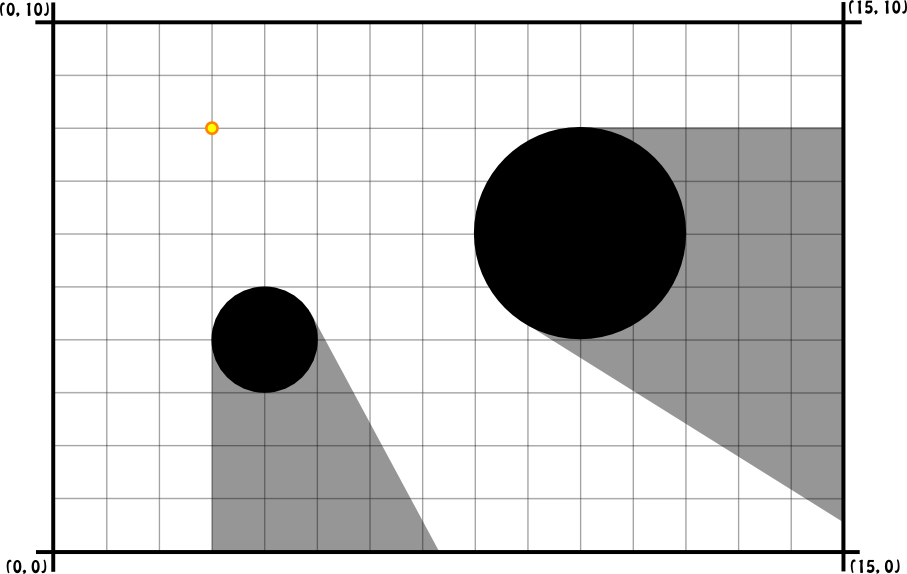
\includegraphics[scale=1.0]{./figuras/bl_1.png}
\end{figure} 

\subsection*{Solución}

Un punto $p$ del perímetro de la pared tiene iluminación si
existe un segmento de línea (un rayo de luz) que comienza en una bombilla de luz, finaliza
en $p$, y no toca o pasa a través de alguna columna. Por tanto:

\begin{itemize}
\item Una cierta porción de la pared está iluminada si alguna bombilla la ilumina (y
no está iluminada si ninguna bombilla la ilumina, es decir, si todas las columnas proyectan una
sombra sobre esta parte de la pared).

\item La sombra que proyecta una columna $c$ a partir de la luz que una bombilla $b$ le incide
queda determinada por las tangentes del círculo descripto por $c$ que que pasan por $b$.
Detrás de la columna (visto desde la bombilla) se proyectará sombra de una
tangente a la otra (si ninguna otra bombilla ilumina esa porción), y
lo demás quedará iluminado (mientras otras columnas no lo impidan).
\end{itemize}

La idea de nuestro algoritmo es calcular las partes de pared que ilumina
cada luz. Para esto recorremos por cada bombilla eléctrica todas las
columnas, y agregamos la sombra que genera cada columna (según la luz
actualmente en consideración) al conjunto de sombras de la bombilla.

Para describir el conjunto de sombras vemos la pared como un único intervalo $(0, 2X + 2Y)$, como
si estuviésemos recorriendo las paredes en sentido antihorario, comenzando desde la pared inferior,
por ejemplo:

\begin{figure}[H]
\centering
\label{bl_2}
\caption{\sc Pared vista como un intervalo en $\mathbb R$}
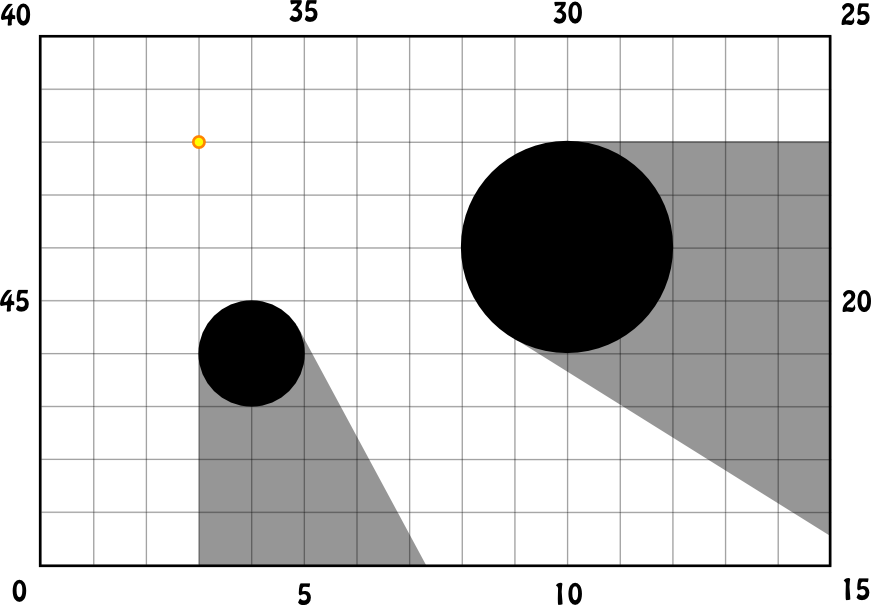
\includegraphics[scale=1.0]{./figuras/bl_2.png}
\end{figure}

Detallamos la traducción de segmentos de pared a un intervalo en la sección
``Cálculo de sombras''. Las sombras resultan entonces subintervalos en $\mathbb R$.
El complemento del conjunto de sombras serán los intervalos de pared iluminada,
y podremos calcular su largo en forma sencilla si los intervalos de este conjunto tienen
intersección vacía. Para esto ``comprimimos'' el conjunto (realizamos la unión
entre intervalos de intersección no vacía).

Unimos todos los conjuntos de intervalos iluminados por las bombillas, formando otro conjunto.
Nuevamente, es simple calcular la longitud de las porciones iluminadas del salón si nos aseguramos que
para este conjunto todos sus elementos tengan intersección vacía. Para esto lo ``comprimimos''
de similar modo que antes, y calculamos el resultado del problema, que es:

\begin{center}
$$\sum_{e\ \in\ intIlum}e_y - e_x$$
\end{center}

Notar que $(\forall\ e \in intIlum)\ e_y > e_x$ por construcción (ver
subsección siguiente, ``cálculo de sombras'').

Para contemplar el error de las operaciones entre flotantes utilizamos un $\epsilon = 0.0000001$, 
de modo que dos flotantes $x_1$ y $x_2$ son considerados iguales si: $abs(x_1 - x_2) < \epsilon$.

\subsection*{Cálculo de sombras}
Dada una luz $L = (l_x, l_y)$ y una columna $C = (c_x, c_y, c_r)$ para calcular la porción sobre
la que se proyecta una sombra consideramos los triángulos que se forman como muestra el siguiente
gráfico:

\begin{figure}[H]
\centering
\label{bl_3}
\caption{\sc Rayos de luz que inciden en la columna}
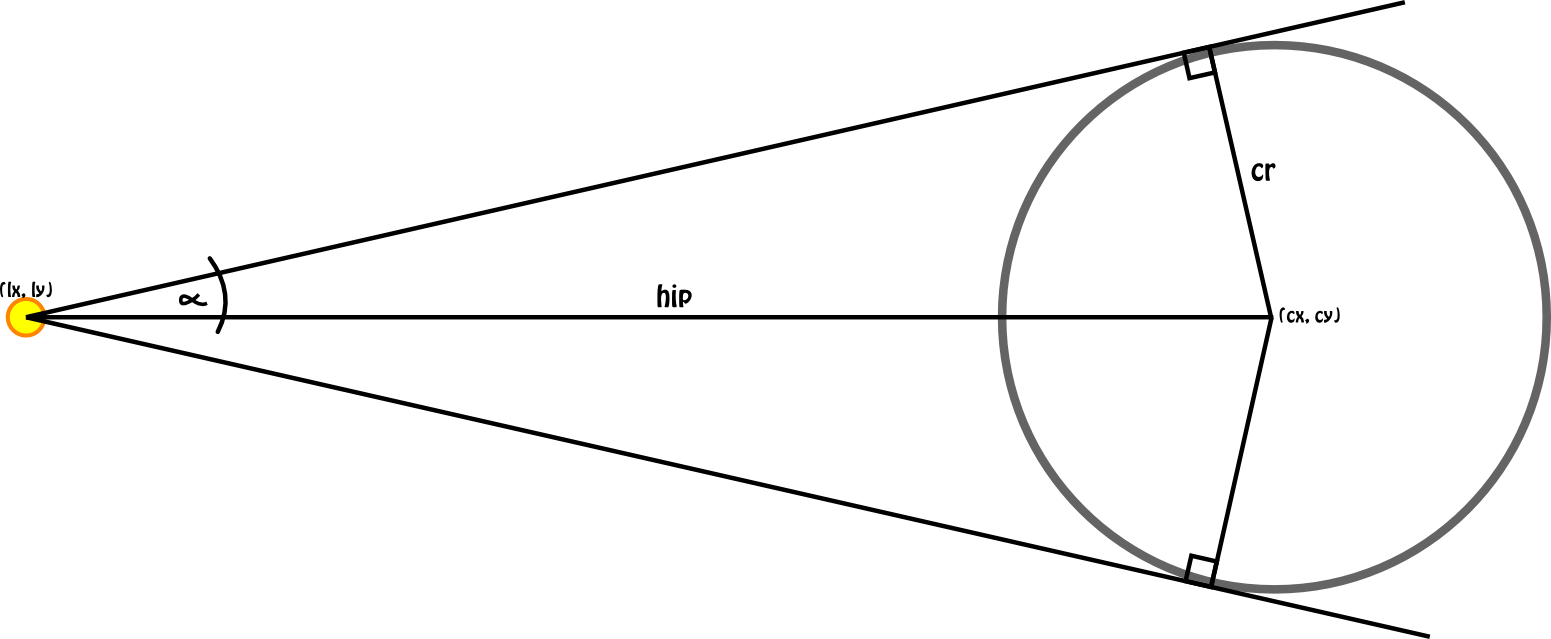
\includegraphics[scale=1.0]{./figuras/bl_3.png}
\end{figure} 

Procedemos de la siguiente forma:

\begin{itemize}
\item Calculamos el vector $v = (c_x-l_x, c_y-l_y)$, que une la luz con el centro de la columna
      (el largo de la hipotenusa es $|v|$).

\item Dado que son triángulos rectángulos, calculamos el seno de alfa como
$\displaystyle\frac{c_r}{|v|}$.

\item Por la igualdad $\sin^2(\alpha) + \cos^2(\alpha) = 1$ obtenemos $\cos(\alpha)$

\item \textbf{Calculamos las tangentes:} rotamos el vector $v$ un ángulo $\alpha$ y un ángulo
$-\alpha$, teniendo en cuenta las propiedades $\sin(-\alpha) = -\sin(\alpha)$ y
$\cos(-\alpha) = \cos(\alpha)$, multiplicando:

\vspace{0.2cm}
\begin{center}
$\left(
\begin{array}{cc}
\cos(\alpha) & -\sin(\alpha) \\
\sin(\alpha) & \cos(\alpha) \\
\end{array}
\right)
v = t_1$
\hspace{1cm}
$\left(
\begin{array}{cc}
\cos(\alpha) & \sin(\alpha) \\
-\sin(\alpha) & \cos(\alpha) \\
\end{array}
\right)  
v = t_2$
\end{center}
\vspace{0.2cm}

esto resulta en dos vectores $t_1$ y $t_2$. A partir de estos vectores consideramos las semirrectas
$st_1$ y $st_2$, ambas de origen $(l_x, l_y)$ y con vectores generadores $t_1$ y $t_2$
respectivamente. Las semirrectas las representamos en su forma vectorial.

\item \textbf{Calculamos los puntos de intersección $(x_1, y_1)$ y $(x_2, y_2)$ de las semirrectas
$st_1$ y $st_2$ respectivamente con los segmentos que representan la pared} (ver sección
``intersección entre semirrecta y segmento'').

\item \textbf{A partir de los puntos de intersección calculamos el intervalo de sombra}
considerando los 4 segmentos de la pared como un único segmento del largo del perímetro,
de la siguiente forma. Sea la función de $R^2 \times R$:

\vspace{0.2cm}
\begin{center}
\[ f(x, y) = \left\{
               \begin{array}{llll}
				 $x$ & \mbox{si $0 \le x < X \wedge y = 0$} \\
				 $X + y$ & \mbox{si $x = X \wedge 0 \le y < Y$} \\
				 $2X + Y - x$ & \mbox{si $0 < x \le X \wedge y = Y$} \\
				 $2X + 2Y - y$ & \mbox{si $x = 0 \wedge 0 < y \le Y$}
			   \end{array}
			 \right.
\]
\end{center}
\vspace{0.2cm}

\end{itemize}

entonces el intervalo de sombra lo definimos como $(f(x_1,y_1), f(x_2,y_2))$ si
$f(x_1,y_1) \le f(x_2,y_2)$, sino definimos la sombra con dos intervalos: $(0, f(x_2,y_2))$ y
$(f(x_1,y_1), 2X + 2Y)$. Este último caso sucede cuando está el punto $(0,0)$ entre las 
semirrectas tangentes.


\subsection*{Intersección entre semirrecta y segmento}

Dada una semirrecta de origen $(x_1, y_1)$ y vector generador $(x_2 - x_1, y_2 - y_1)$ y un
segmento $<(w_1, z_1), (w_2, z_2)>$:

\begin{itemize}
\item Construimos con el segmento una semirrecta de origen $(w_1,z_1)$ y vector generador
$(w_2-w_1, z_2-z_1)$.

\item Calculamos la intersección entre estas semirrectas, y para esto hacemos el mismo cálculo que
para las rectas. Luego restringimos el resultado, de modo que las rectas resultan:

\vspace{0.2cm}
$recta_1 = (x_1, y_1) + t(x_2 - x_1, y_2 - y_1)$

\vspace{0.1cm}
$recta_2 = (w_1, z_1) + s(w_2 - w_1, z_2 - z_1)$
\vspace{0.2cm}

\item Calculamos la intersección entre las semirrectas según el sistema:

$$(x_1 + t(x_2 - x_1), y_1 + t(y_2 - y_1)) = (w_1 + s(w_2 - w_1), z_1 + s(z_2 - z_1))$$

Despejando:

$$s = \displaystyle\frac{(w_1 - x_1)(y_2 - y_1) + (y_1 - z_1)(x_2 - x_1)}
                       {(x_2 - x_1)(z_2 - z_1) - (w_2 - w_1)(y_2 - y_1)}$$

El sistema puede tener única solución, puede no tener solución (si son
rectas paralelas distintas), o puede tener infinitas soluciones (si se
trata de las mismas rectas, una ``encima'' de la otra). En los últimos dos
casos el determinante de la matriz formada por los vectores generadores da 0
(vectores LD):

\vspace{0.2cm}
\begin{center}
$\vline
\begin{array}{cc}
x_2 - x_1 & w_2 - w_1 \\
y_2 - y_1 & z_2 - z_1 \\
\end{array}\vline
= (x_2 - x_1)(z_2 - z_1) - (w_2 - w_1)(y_2 - y_1) = 0$
\end{center}
\vspace{0.2cm}

\end{itemize}

Existe un caso borde en que el determinante es $0$ pero el sistema tiene única
solución. Si las semirrectas tienen el mismo origen pero sentido contrario,
la intersección es el punto de origen. Para saber si tienen sentido contrario
verificamos si el producto interno entre los vectores generadores es negativo.

Si el determinante de la matriz es distinto de cero, la solución es única. Notar
que el determinante es el denominador de $s$, por lo que si este es distinto de
cero, $s$ se puede calcular. Para encontrar el punto de intersección se reemplaza
$s$ en alguna de las rectas con el valor calculado.

Para saber si el punto cae sobre ambas semirrectas verificamos que el producto
interno entre el vector generador de cada semirrecta y el vector que une el
origen de la semirrecta con $p$ es positivo, lo que significa que los vectores
tienen igual sentido que la semirrecta.

Finalmente, dado el punto de intersección, para saber si cae sobre el
segmento resta verificar si el producto interno entre el vector que une el
punto $(w_2, z_2)$ con $(w_1, z_1)$ y el vector que une $(w_2, z_2)$ con $p$
es positivo. Recordemos que no hace falta verificar lo mismo con el vector
que une $(w_1, z_1)$ y $(w_2, z_2)$, pues fue verificado al calcular la
intersección entre las semirrectas (el origen de una de las semirrectas era
$(w_1, z_1)$). Intuitivamente esto es lo mismo que verificar que los vectores
que van desde los extremos del segmento hacia $p$ apuntan ``hacia adentro''
del segmento.


\subsection*{Detalles de Implementación}

Implementamos las siguentes {\bf clases}:

\begin{itemize}
\item[\tt\small Par] Representa un par en $R^2$. Además, para esta
estructura implementamos el operador resta y el de comparación por menor, que es:

$(x_1, y_1) < (x_2, y_2) \Leftrightarrow x_1 < x_2 \vee ( abs(x_1 - x_2) < \epsilon \wedge y_1 < y_2 )$

\item[\tt\small Segmento] Es un par de pares.

\item[\tt\small Semirrecta] Tiene un par que es el origen y un par que es el vector generador.

\item[\tt\small Columna] Tiene tres enteros: $x,y$ que son el centro, y $r$ que es el radio de la columna.

\item[\tt\small Luz] Tiene dos enteros: $x,y$ que es la ubicación de la luz en los ejes $X$ e $Y$.
\end{itemize}

Implementamos los siguentes {\bf métodos}:

\begin{itemize}
\item[\tt\small prodInterno] Devuelve el producto interno de dos pares.

\item[\tt\small interSemirrectas] Dadas dos semirrectas y un par, devuelve un
booleano que indica si existe o no intersección entre las semirrectas. Si
existe intersección la devuelve en el par, en caso contrario no modifica
los valores del par.

\item[\tt\footnotesize interSemirrectaSeg] Dada una recta, un segmento y un par, devuelve
un booleano que indica si existe o no intersección entre la semirrecta y
el segmento. Si existe intersección la devuelve en el par, en caso contrario no
modifica los valores del par.

(Estos dos últimos métodos implementan lo explicado en la sección ``Intersección
entre semirrecta y segmento''.)

\item[\tt\small intervaloSombra] Dado un objeto Luz y un objeto Columna, devuelve
un par que es el intervalo de sombra que proyectan en la pared la Columna y la Luz
pasadas por parámetro. Este método implementa parte de lo explicado en la sección
``Cálculo de sombras'' (no es responsable de ``partir'' el caso particular de
que la primer coordenada del par sea mayor a la segunda).

\item[\tt\small comprimir] Dado un vector de pares con potenciales
intersecciones entre sí, lo devuelve asegurando que todo par de elementos tiene
intersección vacía.

\item[\tt\small complemento] Dado un vector de pares, un valor $min$ y otro
valor $max$, modifica el vector tal que si lo unimos con el vector original,
y luego comprimimos el resultado, sería un par $(min,max)$. Además asegura
que el vector resultado cumple que todo par de elementos tiene intersección
vacía.

\item[\tt\small perimIluminado] Resuelve el problema utilizando los métodos
anteriores (como se explicó en la sección ``Solución'').

\end{itemize}

Representamos la pared con un vector de segmentos de 4 posiciones, las columnas
con un vector de columnas, y las luces con un vector de luces.


\subsection*{Análisis de complejidad}

Los métodos prodInterno, interSemirrectas, interSemirrectaSeg y intervaloSombra
tienen complejidad constante, dado que sólo realizan cálculos matemáticos.

El método comprimir se puede hacer en $O(n\log n)$, siendo $n$ el tamaño
del vector de entrada. Esto es porque al comprimir antes de comenzar a
calcular el resultado ordenamos el vector de entrada ($O(n\log(n))$), luego
recorre linealmente el vector de pares ($O(n)$) construyendo el resultado, y
finalmente modificamos el vector de entrada copiándole el resultado ($O(n)$).

El método complemento también se puede hacer en $O(n\log n)$, pues
utiliza comprimir y luego recorre linealmente el vector de pares ($O(n)$)
construyendo el resultado, y finalmente se modifica el vector de entrada
copiándole el resultado ($O(n)$).

El método perimIluminado es la raíz de todos estos métodos. Este método
recorre todas las luces y por cada luz recorre todas las columnas.

Analizamos el ciclo que recorre todas las columnas: para cada columna
se llama a intervaloSombra, se hace una comparación booleana y se hace {\sl push}
de a lo sumo dos elementos detrás de un vector de pares, por lo que el cuerpo
del ciclo que recorre las columnas tiene complejidad de $O(1)$.

Analizamos el ciclo que recorre todas las luces: para cada luz se recorren
todas las columnas y se genera un vector de pares de tamaño $C$, siendo $C$
la cantidad de columnas, lo que cuesta $O(C\log C)$. Luego hace
{\sl push} de todos los pares resultantes de este complemento en otro vector de
pares (el de porciones iluminadas), lo que tiene complejidad
$O(C)$. Luego se comprime el vector de porciones iluminadas, lo que tiene
complejidad $O(2C\log(2C))$ que es $O(C\log C)$. El vector de porciones
iluminadas tiene un tamaño máximo $C+1$. Esta cota es porque el peor caso
para el tamaño de este vector es una luz y $C$ columnas, lo que como máximo
genera $C+1$ porciones iluminadas. Al agregar luces no agregamos sombras sino
que al contrario, probablemente unimos partes iluminadas, lo que decrementa
la cantidad de partes iluminadas.

Por lo tanto el ciclo que recorre las luces y columnas tiene complejidad
$O(LC\log C)$. El resultado de todo este ciclo es un vector de pares que
representan las porciones iluminadas de la pared.

Finalmente, se recorre este vector de porciones iluminadas ya comprimido, para
aumentar un acumulador que resulta ser la respuesta al problema, lo que tiene
orden $O(C)$.

Por lo tanto, el orden de nuestro algoritmo es $O(LC\log C+C)$, que es $O(LC\log C)$,
siendo $L$ la cantidad de luces y $C$ la cantidad de columnas.
